\documentclass[platz]{tudphygp}
\usepackage{tudphymd,mhchem,listliketab,multirow,tabulary}

\versuch{Nichtleiter im elektrischen Feld}{NF}

\begin{document}
\maketitle

\section*{Aufgabenstellung}
\textbf{Bestimmen Sie die relative Dielektrizit�tszahl $\epsilon_r$ eines vorgegebenen Dielektrikums mit Hilfe eines Zylinderkondensators.}\\
Gehen Sie dabei wie folgt vor:
\begin{enumerate}
 \item Schalten Sie den Oszilloskop und den Generator (kombinierter Sinus- und Kippspannungsgenerator) sofort ein. Bedenken Sie, dass beide 
 Ger�te etwa $\SI{10}{min}$ Einlaufzeit ben�tigen, bevor die f�r die Messungen ben�tigte Stabilit�t erreicht ist.
 \item\textbf{Vorbereitende Messungen mit dem Oszilloskop}
 \begin{enumerate}
  \item Stellen Sie die Impulsform der Kippschwingungen, die mit dem Kippspannungsgenerator f�r Kapazit�ten $C_K\approx (50\dots 600)\SI{}{pF}$ 
  erzeugt werden, mit dem Oszilloskop (Y-Ablenkung, Kanal 1) dar. Benutzen Sie dazu die interne Zeitablenkung (X-Ablenkung) und messen Sie die 
  Schwingungsdauer f�r den Kalibrierkondensator $C_{10x}\approx\SI{110}{pF}$ (den genauen Wert f�r $C_{10x}$ entnehmen Sie der Tabelle 
  \ref{tab:kapa}, $x$-Versuchsplatznummer, $x=1\dots 4$)
  \item Stellen Sie am Sinusgenerator eine Frequenz ein, die der gleichen Schwingungsdauer entspricht und stellen Sie diese Impulsform auf dem 
  Oszilloskop wie unter 2a) (Kanal 2) dar und messen Sie die Schwingungsdauer mit dem Oszilloskop.
  \item Betreiben Sie jetzt den Oszilloskop im X-Y-Mode. Korrigieren Sie geringf�gig die Frequenz des Wechselspannungsgenerators, so dass eine 
  Lissajous-Figur am Oszilloskop zu sehen ist, f�r die die Schwingungsdauer der Kippschwingung mit der der Sinusschwingung �bereinstimmt, 
  und zeichnen Sie diese Figur.
 \end{enumerate}
 \item\textbf{Messungen der Schwingungsdauer der Kippschwingung als Funktion der Kalibrierkapazit�ten des Kippspannungsgenerators}
 \begin{enumerate}
  \item Messen Sie Schwingungsdauer der Kippschwingung als Funktion der Kapazit�t $C_K$ (Werte siehe Tabelle. Welche Kondensatoren ben�tigen 
  Sie zur Kalibrierung?) durch Frequenzvergleich mittels Lissajousfiguren. Weshalb ist dieses Verfahren der direkten Zeitmessung an diesem 
  Oszilloskop vorzuziehen?
  \item Erstellen Sie die Kalibrierungskurve $T=f(C)$.
 \end{enumerate}
 \item Bestimmen Sie mit Hilfe der Kalibrierungskurve und der Messanordnung aus 3. die Kapazit�t eines Zylinderkondensators, der mit einem 
 Dielektrikum gef�llt wird, als Funktion der F�llh�he. Stellen Sie den Zusammenhang grafisch dar.
 \item Ermitteln Sie aus der Grafik die Dielektrizit�tszahl $\epsilon_r$ des Dielektrikums.
\end{enumerate}

\newpage
\section*{Technische Daten}
\parpic[l]{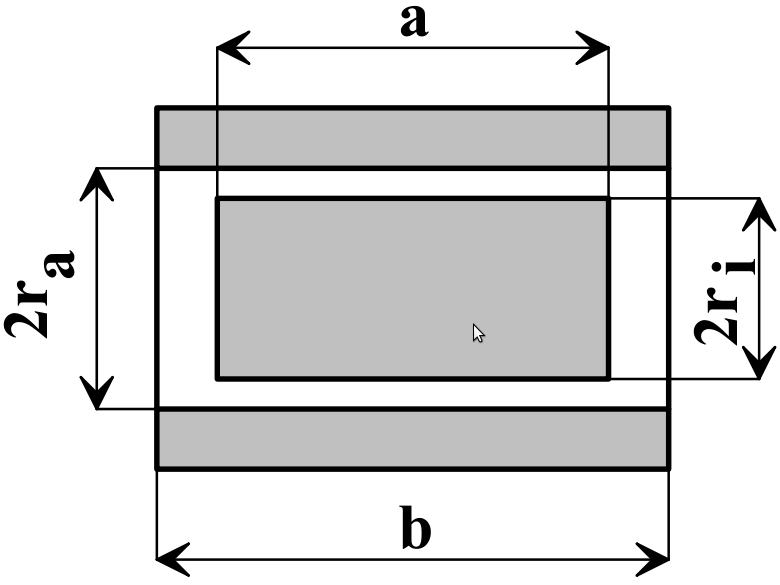
\includegraphics[width=\linewidth/100*35]{abmessungen.png}}
\picskip{3}
Abmessungen des Messkondensators:\\
\storestyleof{itemize}
\begin{listliketab}
 \begin{tabular}{lcl}
  $a$    & $=$ & $\SI{100}{mm}$\\
  $b$    & $=$ & $\SI{110}{mm}$\\
  $2r_a$ & $=$ & $(\num{70,0}\pm\num{0,1})\SI{}{mm}$\\
  $2r_i$ & $=$ & $(\num{65,0}\pm\num{0,1})\SI{}{mm}$
 \end{tabular}
\end{listliketab}
\\\\\\
Der maximale Messfehler der Frequenz des Sinusgenarators ($\SI{200}{MHz}$ SINE-WAVE GENERATOR, Hersteller HAMEG) ist durch die Anzeige dominiert 
und betr�gt $\pm\SI{1}{Digit}$.

\begin{table}[h]
 \centering
 %\scalebox{1.5}{
 \begin{tabular}{|c|c|c|c|c|c|c|}
  \hline
           & \multicolumn{5}{c|}{Kalibrierkapazit�t f�r Kippgeneratoren}                   & Fehler\\\cline{2-7}
           & $C_{n1}$      & $C_{n2}$      & $C_{n3}$      & $C_{n4}$      & $C_{n5}$      & \multirow{2}{*}{$\Delta C/\SI{}{pF}$}\\\cline{2-6}
           & \multicolumn{5}{c|}{$C/\SI{}{pF}$}                                            & \\\hline
  $C_1$    & $593$         & $588$         & $582$         & $600$         & $585$         & $\num{5,9}$\\\hline
  $C_2$    & $489$         & $479$         & $487$         & $505$         & $473$         & $\num{5,4}$\\\hline
  $C_3$    & $415$         & $392$         & $417$         & $420$         & $400$         & $\num{5,0}$\\\hline
  $C_4$    & $341$         & $341$         & $355$         & $329$         & $326$         & $\num{4,7}$\\\hline
  $C_5$    & $284$         & $285$         & $285$         & $286$         & $289$         & $\num{4,4}$\\\hline
  $C_6$    & $215$         & $588$         & $582$         & $600$         & $585$         & $\num{4,1}$\\\hline
  $C_7$    & $\num{197,5}$ & $204$         & $206$         & $207$         & $\num{195,8}$ & $\num{4,0}$\\\hline
  $C_8$    & $\num{168,3}$ & $\num{178,1}$ & $\num{175,6}$ & $\num{184,2}$ & $\num{164,7}$ & $\num{1,2}$\\\hline
  $C_9$    & $\num{152  }$ & $\num{155,8}$ & $\num{150,6}$ & $\num{130,1}$ & $\num{130,3}$ & $\num{1,1}$\\\hline
  $C_{10}$ & $\num{103,9}$ & $\num{110,7}$ & $\num{111,5}$ & $\num{107,4}$ & $\num{112,1}$ & $\num{0,9}$\\\hline
  $C_{11}$ & $\num{ 86,1}$ & $\num{ 77,7}$ & $\num{ 80,6}$ & $\num{ 84,2}$ & $\num{ 79,6}$ & $\num{0,7}$\\\hline
  $C_{12}$ & $\num{ 55,6}$ & $\num{ 55,5}$ & $\num{ 55,4}$ & $\num{ 54,9}$ & $\num{ 54,8}$ & $\num{0,6}$\\\hline  
 \end{tabular}
 %}
 \caption{Werte und Fehler der Kalibrierkapazit�ten des Kippspannungsgenerators}
 \label{tab:kapa}
\end{table}
\end{document}
